% !TeX spellcheck = en_GB

\begin{frame}{\protect{\emoji{thinking-face}} \textit{Deep Learning} in 2022}

\textit{Deep learning} today is a remarkably powerful and mature paradigm, able to reach (super)human-level performance in (selected) \textit{regression}, \textit{classification}, data \textit{generation} and \textit{control} tasks.

\center 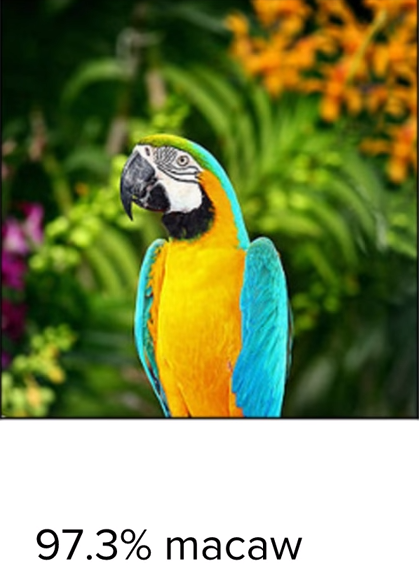
\includegraphics[height=0.35\linewidth]{macaw_macaw.png}
\end{frame}

\begin{frame}{\protect{\emoji{thinking-face}} Also \textit{Deep Learning} in 2022}

    However...

\center 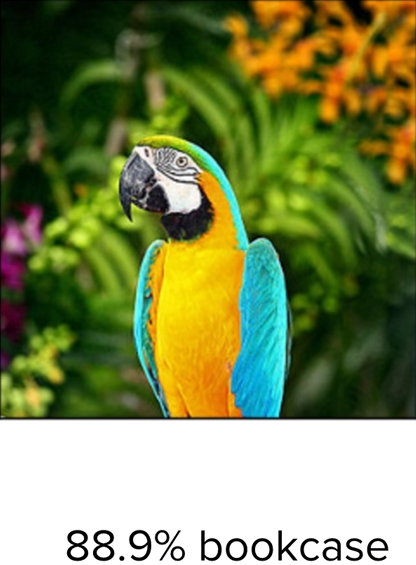
\includegraphics[height=0.35\linewidth]{macaw_bookcase.png}

\hspace*{14px}\textit{(P. Perdikaris, 2018)}
\end{frame}
\setcounter{footnote}{0}

\begin{frame}{\protect{\emoji{thinking-face}} \textit{Adversarial inputs and attacks}}
    The last shown picture is an example of
    \hfill\break
    \begin{block}{\textit{Adversarial Input}}
        An \textit{input} is said to be \textit{adversarial} to a machine learning system if it alters its \alert{reasonably} expected behaviour\footnote{Usually from the \textit{P.o.V.} of the user(s).}. Also called \textit{adversarial attack}, stressing the intentional\footnote{Which is not a strict requirement, though!} crafting of it.
    \end{block}

In the specific case of a classifier: produce a \textit{misclassification}.
\end{frame}


\begin{frame}{\protect{\emoji{thinking-face}} Why studying \textit{adversarial robustness}?}

    We live in times where a growing portion of even \textit{high-stakes} \alert{decisions} is \alert{delegated} to autonomous systems (\textit{e.g.} \textit{HR} selection, insurance, health, fraud detection, \etc\dots).

    \underline{Purely \textit{technical} reasons}
    \begin{itemize}
        \item Harden \textit{ML/DL} systems against \alert{misuse} and \textit{input-tampering};
        \item Assess (and \textit{\alert{patch}!}) behaviour where it the most fragile.
    \end{itemize}

    \underline{\textit{Legal / ethical / social} reasons}
    \begin{itemize}
        \item To ensure \alert{compliance} with regulatory frameworks or coordinated initiatives thereof;
        \item Increase understanding, transparency, and societal \alert{trust}.
    \end{itemize}

    \underline{Broader-reaching goals}
    \begin{itemize}
        \item Use \textit{robustness} as a lens through which to study \textit{\alert{neurocognitive} phenomena}.
    \end{itemize}
\end{frame}

\begin{frame}{\protect{\emoji{thinking-face}} A (more) precise definition of \textit{robustness}}

    We can always reformulate the problem of \textit{adversarial inputs} as one of \textit{\alert{adversarial perturbations}}, \textit{i.e.}
    $$ \vec{x}_{\text{adversarial}} \coloneq  \vec{x}_{\text{legitimate}} + \alert{\vec{p}}$$

    leading to the following

    \begin{block}{Definition: \textit{\alert{$\epsilon$}-perturbative adversarial attack against classifier $\netw{N}$ in $x_0 \in \mathbb{I}$, \wrt $\normof{\cdot}$}}
        Any $\vec{x^{\star}} \coloneq \vec{x_0} + \vec{p} \text{ | } \netw{N}(\vec{x^{\star}}) \neq \netw{N}(\vec{x_0})$ and $\normof{\vec{p}} < \epsilon$
    \end{block}
\end{frame}

\begin{frame}{\protect{\emoji{brain}} \textit{At the end of the day}...}

    No optimal, universal defence! Many \textit{case-by-case} results, many \textit{trade-offs}, practically no \textit{robust-by-design} applicable solution.
    \hfill\break

    \begin{block}{A remark}
        But... have \textit{\alert{you}} ever experienced an \textit{adversarial(-like) phenomenon?}
    \end{block}

\end{frame}
